\documentclass[border=10pt]{standalone}
\usepackage{circuitikz}
\usepackage{tikz}
\usetikzlibrary{calc, positioning, arrows.meta}

\begin{document}
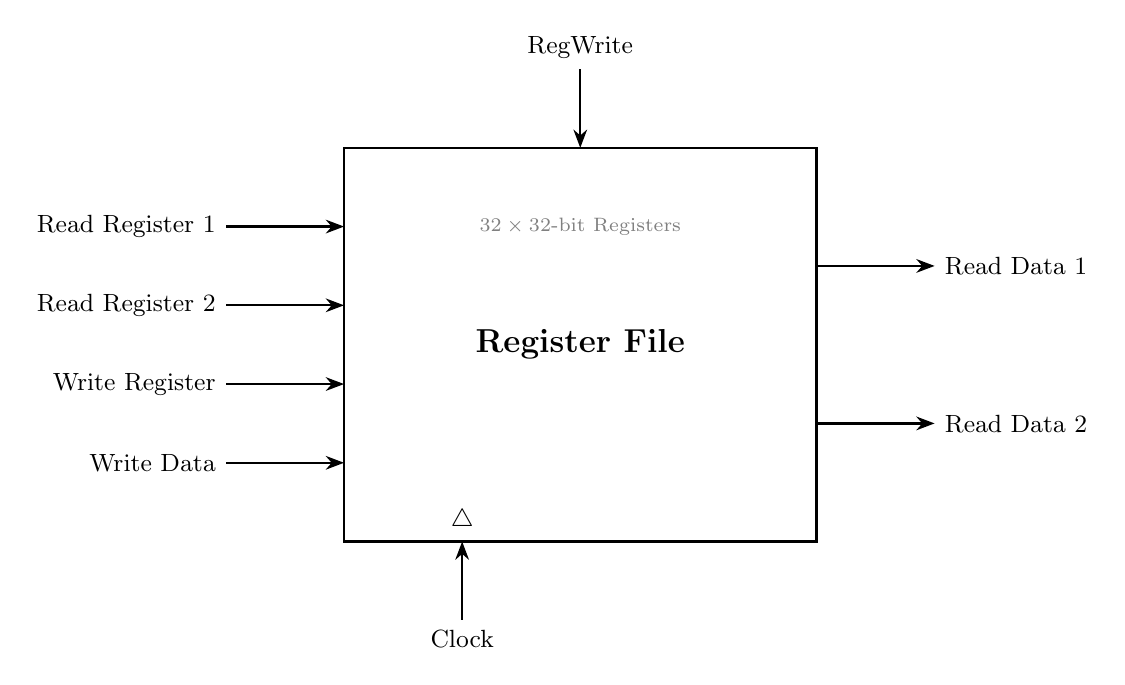
\begin{tikzpicture}[
    >=Stealth, 
    thick, 
    font=\small
]

    % Register File Box
    \draw[fill=white] (0, 0) rectangle (6, 5);
    \node at (3, 2.5) {\large \textbf{Register File}};
    
    % Inputs (Left Side)
    \draw[<-] (0, 4) -- (-1.5, 4) node[left] {Read Register 1};
    \draw[<-] (0, 3) -- (-1.5, 3) node[left] {Read Register 2};
    \draw[<-] (0, 2) -- (-1.5, 2) node[left] {Write Register};
    \draw[<-] (0, 1) -- (-1.5, 1) node[left] {Write Data};
    
    % Control Signals (Top/Bottom)
    \draw[<-] (3, 5) -- (3, 6) node[above] {RegWrite};
    \draw[<-] (1.5, 0) -- (1.5, -1) node[below] {Clock};
    \node[above] at (1.5, 0) {$\triangle$};

    % Outputs (Right Side)
    \draw[->] (6, 3.5) -- (7.5, 3.5) node[right] {Read Data 1};
    \draw[->] (6, 1.5) -- (7.5, 1.5) node[right] {Read Data 2};

    % Internal logic hint (optional)
    \node[gray, font=\scriptsize] at (3, 4) {$32 \times 32$-bit Registers};

\end{tikzpicture}
\end{document}
